\documentclass[12pt, fleqn]{article}

\usepackage[margin=1.0in]{geometry} 
\usepackage{amsmath,amsthm,amssymb}
\usepackage{pgfplots}
\usepackage{tikz}
\usepackage{enumerate}
\usepackage{graphicx}
\usepackage{subcaption}
\usepackage[font=small]{caption}
\usepackage[compact]{titlesec}

\begin{document}

\title{\vspace{-2cm} Predicting TAP Grant Awards: Final Report}
\author{Cean Park (ckp42), Tiffany Shih (ts568)\\
ORIE 4741: Learning with Big Messy Data \\ December 4, 2017}
\date{}

\maketitle

\vspace{-1cm}
\section{Project overview} 
The topic of our study is The New York State Tuition Assistance Program (TAP), New York's largest financial aid grant program. Eligible residents of New York State that attend in-state colleges or universities can apply for the TAP to help pay for their tuition. According to New York's Higher Education Services Corporation (HESC), students may apply for the TAP through the FAFSA, and the award amount is determined by various factors including the academic year in which the first payment of TAP is received, the type of postsecondary institution attended, taxable income, and financial status. 

The goal for our project is to build a model that can accurately predict an applicant's TAP grant award amount given a set of data from his/her TAP application. Through our data analysis, we also hope to determine which fields from a TAP application have the greatest impact on award decisions.

\section{Preliminary Analysis}

\subsection{About the Data}
The data set we are using to complete our analysis is provided by the New York State government. It examines Tuition Assistance Program (TAP) Recipients \& Dollars by Income, Age Group and Program Information for the academic years 2000 to 2015. The data set contains 190,964 examples across 16 features, and stratifies recipients by various factors including age, academic level, type of institution, and financial status. For each stratum, the data set lists the number of TAP recipients and FTEs (Full Time Equivalents) that fall under the aforementioned categories as well as total award amount granted to that group of recipients. In order to make a prediction for a single applicant, we defined a new output feature, ``Average Award Per FTE'', in order to provide an individual rather than aggregate award amount.

The data is composed of a combination of 9 nominal, 5 discrete, and 2 continuous features. Some of the nominal features include Institution Type, Level of Study, and TAP Sector Group. The discrete features include some of our input features, such as ``Income'', ``Year'', and ``Headcount''. Our continuous features are ``Average Award Per FTE'' and ``Average Income'', which is defined in the Data cleaning section below.

From a first glance at the data, the dependency status, age group, sector group, and income level features seem promising as significant variables for prediction.


\subsection{Data Cleaning}
Our goal in cleaning the data was to transform the given TAP recipient data set into entirely numerical values for use in our preliminary model selection. Although there were only 9 nominal variables, many of the other columns in our data were parsed as string objects in the provided CSV file, and thus needed cleaning for usability.

For nominal features, we employed two types of transformations to obtain numerical data:
\begin{enumerate} [(1)]
	\item 
		For nominal features with only two categories, we created a binary column such that a value of 1 represented one category and a value of 0 the other. This was done for the “TAP Level of Study,” “Sector Type,” “TAP Financial Status,” and “Degree/Nondegree” features.
	\item
		For nominal features with more than two categories, we used one-hot encoding transform a feature with k categories into k binary-valued columns. This was applied to the other 5 nominal features.

\end{enumerate}

Although most of the discrete/continuous features were encoded as numbers in the data, the Income features were provided in the data as strings describing the range of income, e.g. ``\$2,001 to \$3,000''. We decided to numerically represent the income range as the average of the endpoints, so we wrote a function to parse each endpoint and return the average; this feature was labeled as ``Average Income''.

By using the $isna$ function, we found that the provided data set surprisingly only had two missing values, both of which were in the ``TAP Recipient FTE'' column. Since both missing values corresponded to ``Headcount'' values of 1, and each headcount can either be equal to 0.5 or 1 FTE, we replaced both empty values with the average of the two, 0.75.

Lastly, we removed the ``Headcount'', ``FTE'', and ``Dollars'' columns (since these features describe the aggregate applicant pool) and added an offset column for a total of 42 columns in our data set.

\begin{figure}
	\begin{center}
	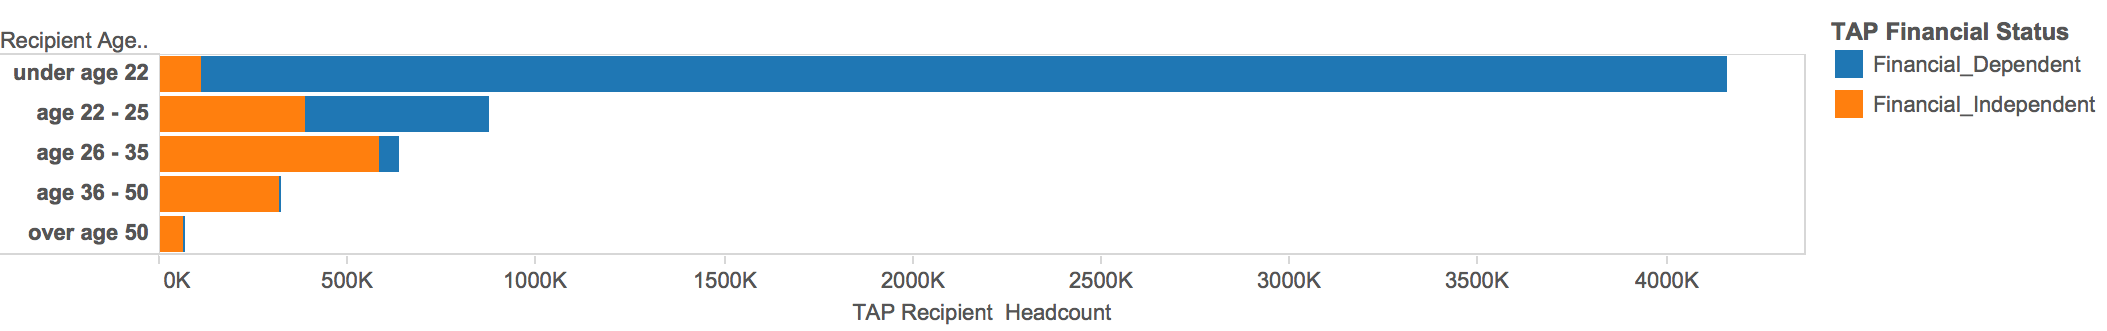
\includegraphics[scale = 0.30]{financial_status.png}
	\caption{Recipient Demographic by Age and Financial Status}
	\end{center}
	\begin{minipage}[c]{0.4\linewidth}
		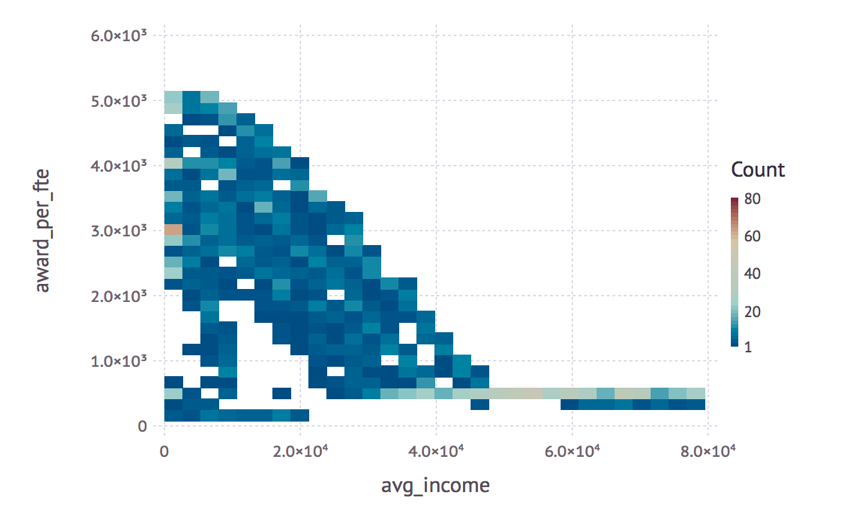
\includegraphics[width=\linewidth]{avgincome_vs_award.png}
		\caption{2-D Histogram of Grant Award per FTE vs. Income}
	\end{minipage}
	\hfill
	\begin{minipage}[c]{0.5\linewidth}
		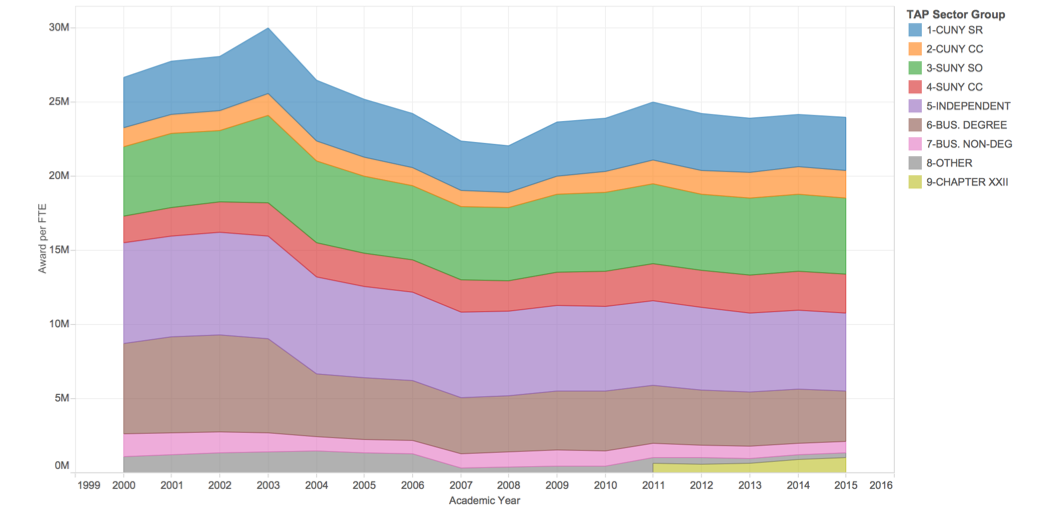
\includegraphics[width=\linewidth]{sector_group.png}
		\vspace{-0.5cm}
		\caption{Sum of TAP Awards from 2000-2015 by Sector Group}
	\end{minipage}
\end{figure}

\subsection{Exploratory Data Analysis}
In order to achieve a better understanding of our data, we explored various summary statistics and visualizations. First and foremost, we wanted to understand what kind of demographic we were working with (see Figure 1). It is evident through this bar graph that the major demographic of TAP recipients consists of students under the age of 22 who hold financial dependent status. This is consistent with our assumptions of the population.

In addition to demographic, we wanted to observe which variables might carry a heavier weight in the grant award decision, and intuitively, we thought that might be a recipient's average income. Due to the vast amount of examples that we have in the data set, we took a simple random sample of 1,910 examples to generate our visualization.

From our histogram (see Figure 2), it is evident that there is some correlation between average income and grant award. In general, as average income increases, grant award decreases. However, it is interesting to note that the award granted to recipients with average income over \$50,000 is capped at around \$500, while there is great variability within the awards granted to recipients in the lower average income regime. This could indicate that there is another variable that significantly influences grant award decision, especially for low average income recipients.

Another aspect of the data we were curious about was the variability of TAP awards from year to year. Plotting these (see Figure 3), it seems that there is a notable increase in total awards granted from 2000 to a peak in 2003 and a notable decrease from 2003 to a low in 2008. This low point could perhaps have been influenced by the recession of '08. We also wanted to add another dimension to this visualization to see if students enrolled in a certain category of NYS colleges/universities received more or less grant awards than others. It seems that state-operated SUNY schools as well as independent colleges receive a larger fraction of the total grant pool. 

In addition to these visualizations, a couple notable summary statistics include the mean and median grant award amounts, which are \$2,101.76 and \$2,033.33 respectively. Given that TAP recipients can be awarded up to \$5,165 annually, it seems that it is more common for recipients to receive less than half the total potential award amount. This could be due in part to the \$500 cap that we noticed for those in the upper half of the average income range.


\section{Model Selection and Results}
Prior to selecting our models for analysis, we partitioned our cleaned data set into training (60\%), validation (20\%), and test (20\%) sets. In addition, we chose to measure the error of our models via mean absolute error (MAE) and mean absolute percentage error (MAPD). The equations for these error calculations can be found below:
\begin{align*}
	MAE &= \tfrac{1}{n} \sum_{i=1}^{n} |y_i - x_i| & \text{where $y_i$ is predicted and $x_i$ is actual} \\
	MAPD &= \tfrac{100}{n} \sum_{i=1}^{n} |\tfrac{y_i - x_i}{x_i}| & \text{where $y_i$ is predicted and $x_i$ is actual}
\end{align*}

We remained consistent with the use of these error calculations throughout our analysis in order to compare and contrast the effectiveness of our models.


\subsection{Quadratic Loss Models}
\subsubsection{No Regularizer}
	The first model we ran was a simple linear regression without any regularizers to use as our baseline model. To do this, we minimized the quadratic loss function: $|| y - Xw ||^2$, where $y$ contains the true outputs, $X$ our training data, and $w$ our model coefficients. By doing so, we wanted to see if there was a linear correlation between the 42 features of our data set and TAP award amount granted to a particular individual.

	Our linear regression with quadratic loss yielded validation set errors of: 510.6442 (MAE) and 62.6073\% (MAPD). 

	Due to the large error obtained from this linear regression, we are not confident that a linear model is a good fit for this data. We believe instead that the linear model severely underfits - and likely speaks to the nonlinear nature of the data set itself.


\subsubsection{Ridge Regression}
	Interested to see how regularization would affect our model, we chose to fit ridge regression to our data set. Ridge regression or quadratically regularized least squares, seeks to minimize the same quadratic loss function plus the quadratic regularizer: $|| y - Xw ||^2 + \lambda ||w||^2$, where $\lambda > 0$. 

	In adding a regularizer to the objective function, we can stabilize our estimates and produce a unique solution. In particular, the quadratic regularizer adds a small penalty for large coefficients and therefore shrinks coefficients towards 0 such that the solution becomes less sensitive to small changes in the data. 

	We trained a model with regularization parameter $\lambda = 0.25$ and obtained errors of: 510.6451 (MAE) and 62.6068\% (MAPD). 

	The errors we obtained from this ridge regression were very similar to the results we obtained from the initial linear regression which may be intuitive, since our initial linear model had underfit the data, it does not seem that regularization helps in reducing the error.


\subsubsection{Lasso Model}
	In addition to the ridge regression model, we were interested to see how the $l$-1 regularizer would fit the data. Since the $l$-1 regularizer encourages sparsity in the coefficients, we thought it may be interesting to see which features were the most important in determining TAP grant award amount. The objective of this lasso model is as follows: minimize $|| y - Xw ||^2 + \lambda \sum_{i=1}^{d} |w_i|^2$, where $d$ represents the number of features in the data set. 

	In order to select an appropriate lambda parameter for this model, we used cross-validation. We found the optimal lambda value to be 0.0033. Since this value is close to 0, we believed that this model would yield results similar to the simple linear regression model, which would support our hypothesis that regularization does not help in this case to reduce the error of our already underfit linear model.

	Our lasso model yielded a validation MAE of 510.6499 and validation MAPD of 62.6077\%. Again, the errors we obtained were very similar to those obtained in the linear and ridge regression models. 

	Looking further into the coefficients obtained through lasso, we saw that 6 of the 42 coefficients had values of 0.0. Comparing these with the columns of TAP data, the results of the model imply that the following features do not matter as much in the determination of an individual's TAP grant award: \textit{Level 2} (Undergraduates in a 2 year program of study), \textit{Group 5} (Independent Colleges), \textit{Age 26-35}, \textit{Award Schedule Letter H} (Students at non-degree institutions and for profit registered schools), and \textit{Award Schedule Letter V}. This could mean that students in shorter terms of study or non-degree granting programs as well as students in private institutions do not receive a significant amount of aid from New York State through the TAP program.

	As a result of our analyses of these models, we do not believe there to be a strong linear relationship between the features in our data set and the average TAP grant award amount. Therefore, as we continued our analysis, we chose to explore a few nonlinear models.

\subsubsection{Polynomial Regression}
	Given that our analysis using linear models yielded inconclusive results, we thought to fit a polynomial model to the data. Since we believe average taxable income to be a very significant feature in the determination of grant awards, we added an additional column within our data set of ${AverageIncome}^2$. Using this expanded data set, we ran regression again and found the following errors on the validation set: MAE: 425.5776, MAPD: 49.3206\%. 
	
	The errors we obtained were lower than those of the previous linear models, but were still very large. This shows that though this polynomial model provides a better fit than the previous linear models, we still need to further explore other nonlinear models to find a best fit.


\subsection{Regression Tree Models}

\subsubsection{Full Tree}
	A regression tree is a type of decision tree that attempts to predict a continuous response variable (in our case, the Award per FTE for a given input.) This technique first partitions the feature space into $N$ non-overlapping regions $R_1, \dots, R_N$, in which each partition represents a split on a single feature variable, e.g. $R_1 = \{ X | X_j \leq s\}$ and $R_2 = \{X | X_j > s\}$. This technique is often referred to as a tree since the partitioning can be represented as a binary tree, with each subtree representing a feature split. Each partition $R_i$ then returns the prediction $\hat{y}_{R_i} = \tfrac{1}{n} \sum_{j\in R_i} y_j$, where $n$ is the number of training observations in $R_i$ and $y_j$ is the true output from the training data. The partitioning of the feature space is done via recursive binary splitting, a greedy approach that attempts to find the feature $j$ and cutpoint $s$ to split upon at each level of the tree (without looking ahead) that minimizes the residual sum of squares. 

	Figures 4 and 5 show an example of a regression tree model and its associated partitions for a two-feature data set.

	We expect a regression tree to overfit the data since as the number of feature space partitions increases, the tree is more likely to ``memorize'' the training data and thus fail to generalize on a validation or test set.

	\begin{figure}
	\begin{minipage}[c]{0.4\linewidth}
		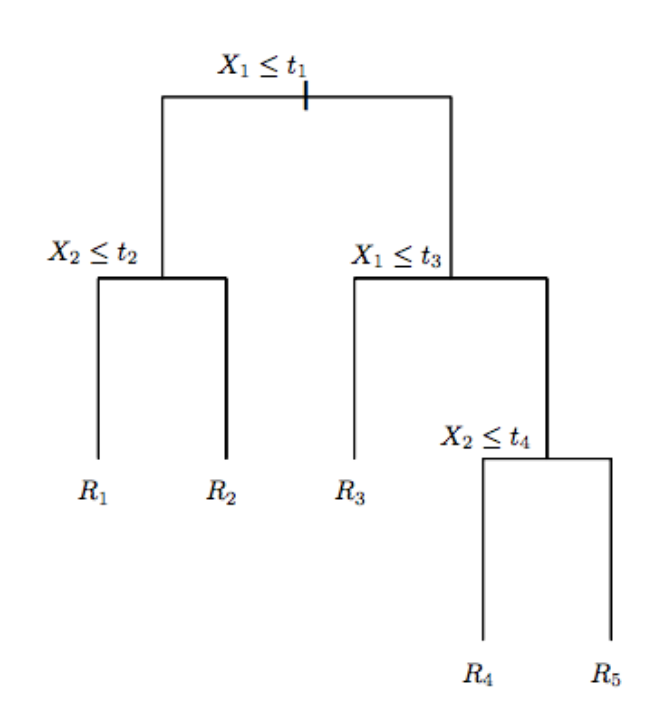
\includegraphics[width=\linewidth]{regr_tree1.png}
		\caption{Tree depiction of regression tree with two features}
	\end{minipage}
	\hfill
	\begin{minipage}[c]{0.4\linewidth}
		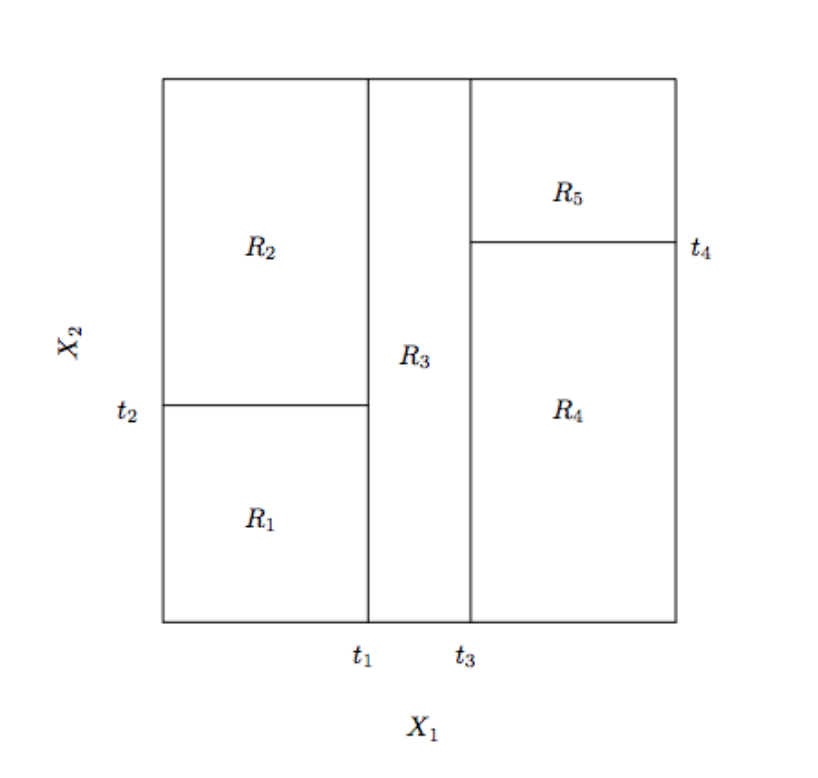
\includegraphics[width=\linewidth]{regr_tree2.png}
		\caption{Visual depiction of corresponding feature space partitions}
	\end{minipage}
	\end{figure}

	Using a regression tree with an average nodes per leaf parameter of 10, we obtained a tree with 21852 leaves and a depth of 80 nodes. Testing this tree against our validation set, we obtained a MAE of $0.0915$ and a MAPD of $0.0096\%$. These results are promising, as the MAE is 4 orders of magnitude better than that of any of the linear models, and the MAPD is significantly smaller. This result seems to imply that there exist certain combinations of features that reliably get a certain TAP grant award amount, i.e. certain types of applications submitted to the TAP correspond to specific award amounts.
	

\subsubsection{Pruning}
	Pruning is a technique that attempts to remedy the overfitting nature of regression trees by ``collapsing'' certain leaves of the tree to reduce its depth and complexity (and thus avoid memorizing the training data.) Pruning can either take a top-down approach or bottom-up approach, all with their pros and cons. Some of the most popular pruning techniques include cost-complexity pruning, which attempts to optimize both the misclassification error against the total number of leaves of the tree, and purity pruning, which prunes leaves based on some purity (correctness) threshold.

	We pruned the obtained regression tree above with a pruning purity parameter of 0.95, which means that leaves were collapsed if the corresponding parent leaf predicted the true output with an accuracy greater than or equal to 0.95. This pruned regression tree had 12319 leaves and a depth of 25 nodes, a significantly less complex tree than the previous one. Corresponding validation set errors were: 0.0919 (MAE) and 0.0096\% (MAPD), almost identical to that of the previous tree. 

	Since we obtained almost-identical performance on the pruned tree, it seems that our pruning tree model is more favorable than the full tree, since it is less complex (less leaves and nodes). Again, the similar performance to the full tree model strengthens the hypothesis that there exist certain subsets of applications (corresponding to leaves of the tree) that receive very similar TAP grant award amounts.


\subsubsection{Random Forest}
	Another technique to remedy the overfitting nature of decision trees is random forest, which ensembles trees together to obtain a joint prediction. Parameters for building a random forest model include: number of trees, number of features per tree (how many randomly selected features to build a decision tree upon), average number of nodes per leaf (as described in the Full Tree section), and portion of samples per tree (which represents how much of the training set to randomly sample to build each tree). Random forests make predictions by taking the average prediction across all trees in the forest.

	Randomly selecting only a fraction of the training set data and features allows for faster computation, but more importantly utilizes the ``ensemble'' nature of trees: the idea that a collection of multiple trees, each trained on an incomplete data set, can make a joint prediction better than that of a single tree trained on a complete data set. 

	We built a random forest of 30 trees, each tree containing around half (20) of the features and using 70\% of the training data with an average of 50 examples per leaf. Our 30-tree ensemble contained an average of 3088.23 leaves and had an average depth of 38.1 nodes. This model achieved validation set errors of 4.6368 (MAE) and 0.4388\% (MAPD) respectively.

	Although we expected the random forest to be the regression tree model that performed the best on the vaildation set, our results clearly show it is the worst performing across the three. We hypothesize that perhaps our 4 parameters for the random forest (number of trees, number of features per tree, average nodes per leaf, portion of samples per tree) need more fine tuning to obtain a better model. It is important to keep in mind that although the random forest was the worst performing decision tree-based model, it still performed significantly better than any of the linear models tested.


\subsection{Final Model Testing}
After using the training (60\%) and validation (20\%) sets to obtain several models, we decided to test the three decision tree based models on our final test (20\%) set. 

Our lowest error model was our full tree model (with 10 nodes per leaf on average), obtaining test set errors of 0.0888 (MAE) and 0.0172\% (MAPD). The next best was the pruned tree model, with test set errors of 0.0891 (MAE) and 0.0173\% (MAPD). Like on our validation set, our random forest model performed the worst, with MAE and MAPD test set errors of 4.5785 and 0.4729\% respectively.

\section{Conclusion}
\begin{figure}
	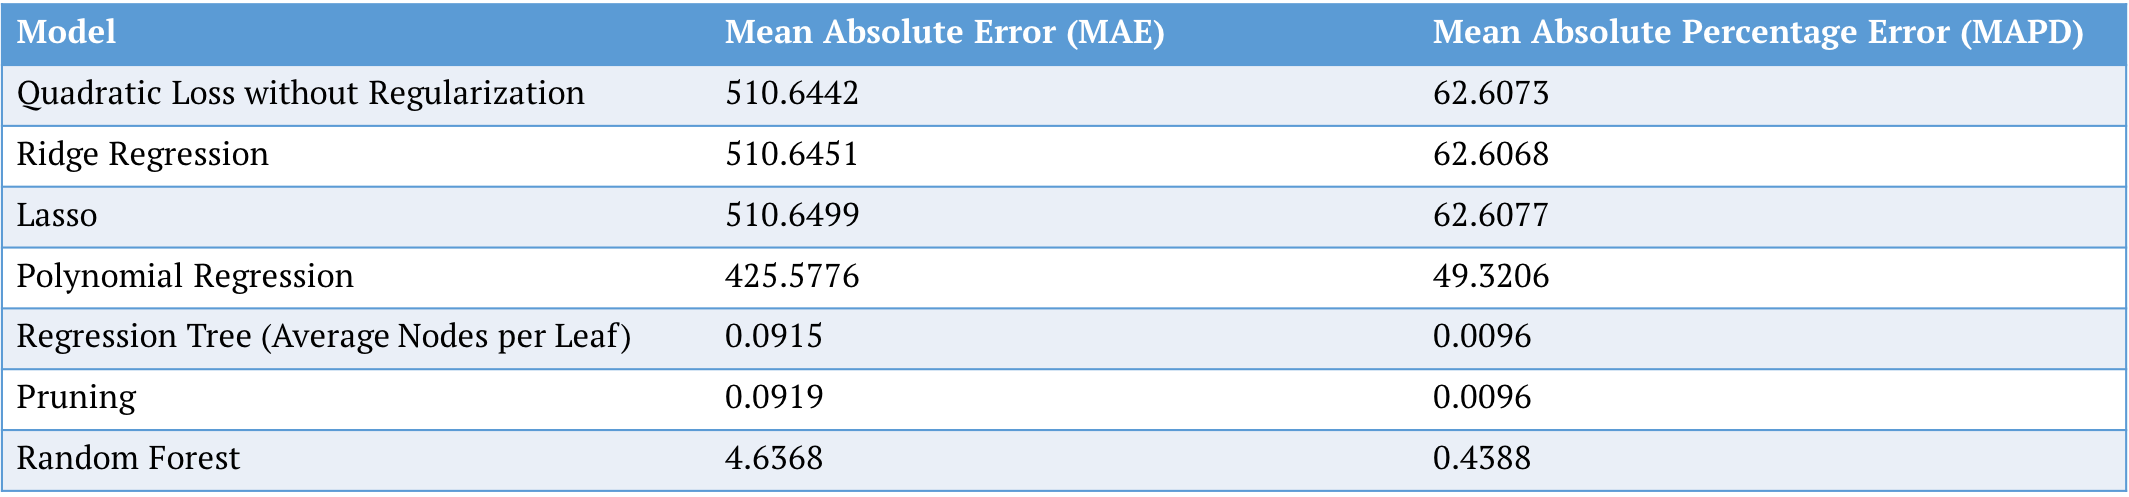
\includegraphics[scale = 0.5]{Errors.png}
	\caption{Trained models and associated validation set errors}
\end{figure}


To summarize, through this analysis, we sought to tackle the problem of predicting TAP grant award amounts when given a candidate's application data. After cleaning and exploring the data set, we split our data into training, validation, and test sets to measure the effectiveness of various models. We first chose to fit a regression model without regularization to use as our baseline model and then moved on to more complex models, including those with regularization as well as those that are nonlinear. From the linear and regression tree models tested, there was a significantly lower error for the regression tree models (full tree, pruned, random forest.) These results tell us that the relationship between TAP application fields and TAP grant award amount is nonlinear and requires more complexity and flexibility than a linear model to fit the data well. 

The model that we recommend New York State to use is our pruned tree model, since it is less complex than the full tree model while having nearly identical validation and test set errors. We are fairly confident in this model, as the errors obtained are objecively low. Some next steps we recommend to further validate our model would be to test this model on the 2016 TAP grant award data that is exepected to be released at the end of this year.


\end{document}

